% Created 2017-08-31 Thu 12:28
% Intended LaTeX compiler: pdflatex
\documentclass[presentation]{beamer}
\usepackage[utf8]{inputenc}
\usepackage[T1]{fontenc}
\usepackage{graphicx}
\usepackage{grffile}
\usepackage{longtable}
\usepackage{wrapfig}
\usepackage{rotating}
\usepackage[normalem]{ulem}
\usepackage{amsmath}
\usepackage{textcomp}
\usepackage{amssymb}
\usepackage[font=small,labelfont=bf]{caption}
\usepackage{hyperref}
\usepackage{booktabs, dcolumn}

\usepackage{tikz}
\usetikzlibrary{arrows, shapes} 
\usetikzlibrary{backgrounds}
\usetikzlibrary{fit}
\usepackage{pgfplots}
\tikzstyle{every picture}+=[remember picture]
\everymath{\displaystyle}

\usetheme{Darmstadt}
\usecolortheme{beaver}
\usefonttheme{structurebold}
\author{Thomas de Graaff}
\date{May 25, 2018}
\title{Spatial Stochastic Frontier Models}
\subtitle{On spatial dependence in stochastic frontier models with an application to European regional economic performance}
\institute[INST]{Department of spatial economics, Vrije Universiteit Amsterdam\\\url{http://www.thomasdegraaff.nl/} \newline\newline Package development at \newline\url{https://github.com/Thdegraaff/SpatFrontier/}}
\setbeamertemplate{navigation symbols}{}
\hypersetup{
	pdfauthor={Thomas de Graaff},
	pdftitle={Spatial Stochastic Frontier Models},
	pdfkeywords={},
	pdfsubject={},
	pdfcreator={Emacs 25.2.1 (Org mode 9.0.10)}, 
	pdflang={English}}
\begin{document}
	
\maketitle
	
\section{Why bother?}

\subsection{Regional economic performance}

\begin{frame}
\frametitle{Regional economic performance}
\framesubtitle{GDP per capita across Europe in 2007---EU27 = 100 (source: cambridge econometrics database}
\begin{columns}
	\begin{column}{0.7\columnwidth}
		\begin{center}
			\begin{figure}[h]
				\center
				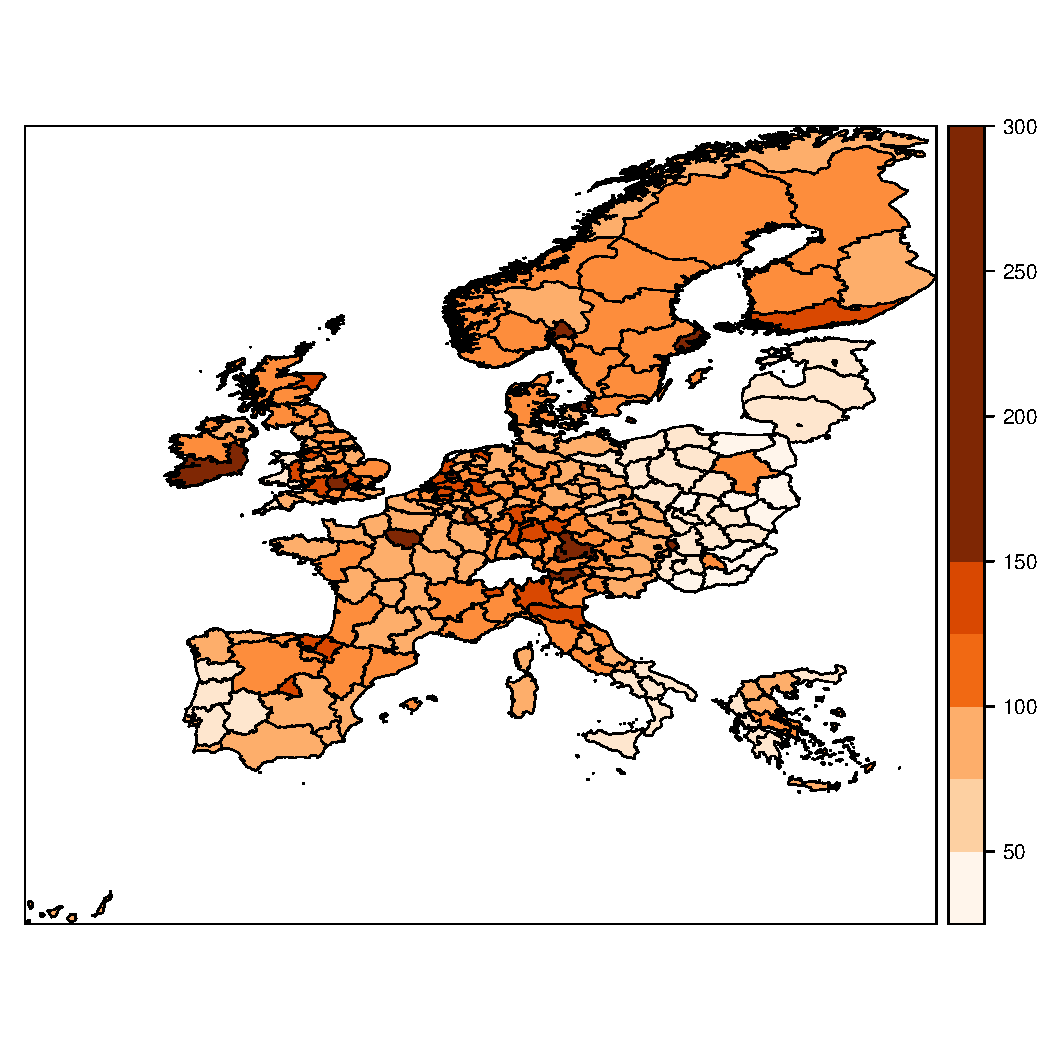
\includegraphics[width=0.9\textwidth]{gdppc}
			\end{figure}
		\end{center}
	\end{column}
	\begin{column}{0.3\columnwidth}
		Huge differences between and within countries
		\begin{itemize}
			\item Different use of endowments
			\item Different relative location within the network
		\end{itemize}
	\end{column}
\end{columns}
\end{frame}

\begin{frame}{Production function isoquant}
\tikzstyle{background}=[circle, fill=gray!30,inner sep=0.5cm]
\begin{center}
	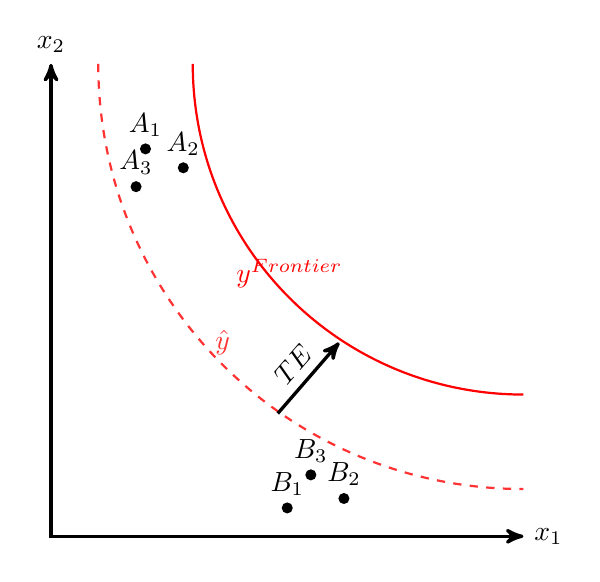
\begin{tikzpicture}[
	scale = 1.2,
	frontier/.style={red,thick},
	axis/.style={very thick , ->, >=stealth', line join=miter},
	region/.style={circle, fill=black, minimum size=4pt, inner sep=0pt, outer sep=-1pt},
	]
	
	\draw[axis,<->] (5,0) node(xline)[right] {$x_1$} - | 
	(0,5) node(yline)[above]{$x_2$};
	\draw[frontier] (1.5,5) to[out=270,in=180] node[above]  {$y^{Frontier}$} (5,1.5) ;
	\node (A1) [region,label=above:$A_1$] at (1,4.1) {};
	\node (A2) [region,label=above:$A_2$] at (1.4,3.9) {};
	\node (A3) [region,label=above:$A_3$] at (0.9,3.7) {};
	\draw[frontier, red!80, dashed] (0.5,5) to[out=270,in=180] node[above]  {$\hat{y}$} (5,0.5);
	\node (B1) [region,label=above:$B_1$] at (2.5,0.3) {};
	\node (B2) [region,label=above:$B_2$] at (3.1,0.4) {};
	\node (B3) [region,label=above:$B_3$] at (2.75,0.65) {};
	\draw[->, very thick, black, >=stealth'] (2.4,1.3) -- (3.05,2.05)
	node[sloped, above, midway] {$TE$};
	\end{tikzpicture}
\end{center}
\end{frame}

\begin{frame}{Production function isoquant with spatial dependence}
\tikzstyle{background}=[circle, 
fill=gray!30,
inner sep=0.5cm]
\begin{center}
	\begin{tikzpicture}[
	scale = 1.2,
	frontier/.style={red,thick},
	axis/.style={very thick , ->, >=stealth', line join=miter},
	region/.style={circle, fill=black, minimum size=4pt, inner sep=0pt, outer sep=-1pt},
	]	
	\draw[axis,<->] (5,0) node(xline)[right] {$x_1$} - |
	(0,5) node(yline)[above]{$x_2$};
	\draw[frontier] (1.5,5) to[out=270,in=180] node[above]  {$y^{Frontier}$} (5,1.5) ;
	\node (A11) [region,label=above:$A_1$] at (1,4.1) {};
	\node (A21) [region,label=above:$A_2$] at (1.4,3.9) {};
	\node (A31) [region,label=above:$A_3$] at (0.9,3.7) {};
	\draw[frontier, red!30, dashed] (0.5,5) to[out=270,in=180] node[above]  {$\hat{y}$} (5,0.5);
	\draw[frontier, red!80, dashed] (1,5) to[out=270,in=180] node[above]  {$\hat{y_A}$} (5,0.75);
	\draw[frontier, red!80, dashed] (0.1,5) to[out=270,in=180] node[above]  {$\hat{y_B}$} (5,0.2);
	\node (B11) [region,label=above:$B_1$] at (2.5,0.3) {};
	\node (B21) [region,label=above:$B_2$] at (3.1,0.4) {};
	\node (B31) [region,label=above:$B_3$] at (2.75,0.65) {};
	\draw[->, very thick, black!30, >=stealth'] (2.4,1.3) -- (3.05,2.05)
	node[sloped, above, midway] {$TE$};
	\draw[->, very thick, black!80, >=stealth'] (1,2.3) -- (2,3.1)
	node[sloped, above, midway] {$TE_B$};
	\draw[->, very thick, black!80, >=stealth'] (3.91,0.89) -- (4.2,1.6)
	node[sloped, above, midway] {$TE_A$};
	\begin{pgfonlayer}{background}
	\node[background, fit =(B11) (B21) (B31), label=left:Country $B$]{};	
	\node[background, fit =(A11) (A21) (A31), label=right:Country $A$]{};	
	\end{pgfonlayer}
	\end{tikzpicture}
\end{center}
\end{frame}

\subsection{Related literature}

\begin{frame}{Related literature}
\begin{itemize}
	\item Starting point: Weinstein (Technometrics, 1964)
	\begin{itemize}
		\item Econometric literature: Aigner et al. (1977); Meeusen \& van den Broeck (1977). 
		\item Statistical literature: Azzalini (1985); Azzalini \& Capitanio (1999); Dominguez-Molina et al. (2003)
	\end{itemize}
	\pause
	\item Regional stochastic frontiers: Puig-Junoy (2001); Alvarez (2007)
	\pause
	\item Recent literature concerning spatial stochastic frontiers: 
	\begin{itemize}
		\item Parametric approach: Pavlyuk (2010); Barrios \& Lavado (2010); Fusco \& Vidoli (2013); Kinfu \& Sawhey (2015); Glass et al. (2016); Jiang et al. (2017)
		\item Bayesian approach/sampling: Schmidt et al. (2009); Areal et al. (2012); Tsionas \& Michealides (2016)
	\end{itemize}
	\pause
	\item Two \texttt{R}-packages:
	\begin{itemize}
		\item \texttt{ssfa}---Fusco \& Vidoli (2015)
		\item \texttt{spfrontier}---Dmitry Pavlyuk (2016)
	\end{itemize}
\end{itemize}
\end{frame} 

\section{Spatial stochastic frontiers}

\subsection{The stochastic production frontier model}

\begin{frame}{Stochastic production frontiers}
\tikzstyle{na} = [baseline=-.5ex]
In general, regional production,$y$, can be modeled as:
%
\begin{equation*}
y = f(\mathbf{X};\beta)TE,
\label{productionfrontier}
\end{equation*}
%
Assume Cobb-Douglas and $TE = \exp(-\mu)$, then:
%
\begin{equation*}
\ln y = \ln(\mathbf{X}) \beta 
\underbrace{
-
\tikz[baseline]{
	\node[fill=red!20, ellipse,anchor=base] (t2)
	{$\mu $};
}
+
\tikz[baseline]{
	\node[fill=green!20, ellipse,anchor=base] (t3)
	{$\nu$};
}
}_{\epsilon = \text{Observed residuals} },
\label{specification}
\end{equation*}
%
Where usually:
\begin{itemize}
	\item $\mu \sim N^+ \left(0,\sigma^2_\mu\right)$ so $\mu \geq 0$
	\item $\nu \sim N \left(0,\sigma^2_\nu\right)$
\end{itemize}
and $\nu$ and $\mu$ are independent of each other 
\end{frame}

\begin{frame}{Tradional (econometric) approach}
	For likelihood purposes one usually considers the composite stochastic variable $\epsilon = \nu - \mu$ en then find the marginal density of $\epsilon$:
	%
	\begin{eqnarray}
	f(\epsilon)	&=& \int_0^\infty f(\mu, \epsilon)d\mu \notag\\
	&=& \frac{2}{\sigma}\phi\left(\frac{\epsilon}{\sigma}\right)\Phi\left(-\frac{\epsilon\lambda}{\sigma}\right)
	\label{likelihood}
	\end{eqnarray}
	%
	Technical efficiencies can be retrieved by $f(\mu|\epsilon)$. 
\end{frame}

\begin{frame}{Imposing spatial structure}
\framesubtitle{A typology}
Note that $\mathbf{A} = \left(\mathbf{I} - \lambda\mathbf{W}\right)$ and $\mathbf{B} = \left(\mathbf{I} - \rho\mathbf{W}\right)$
	\begin{enumerate}
		\item Spatial dependence in technical efficiency component $\mu$
		\begin{equation*}					
			\ln y = \ln(\mathbf{X}) \beta \underbrace{- \mathbf{A}^{-1}\mu + \nu}_\epsilon
		\end{equation*}
		\item Spatial dependence in error term $\nu$:
		\begin{equation*}					
			\ln y = \ln(\mathbf{X}) \beta \underbrace{- u +  \mathbf{A}^{-1}\nu}_\epsilon
		\end{equation*}
		\item Spatial lag separate from technical efficiency component $\mu$
		\begin{equation*}					
			\ln y =  \mathbf{B}^{-1}\left[\ln(\mathbf{X}) \beta\right] \underbrace{+ \mathbf{B}^{-1}\nu - \mu}_{\epsilon}
		\end{equation*}
		\item Spatial lag
		\begin{equation*}					
			\ln y = \mathbf{B}^{-1}\left[\ln(\mathbf{X}) \beta \right]+  \underbrace{\mathbf{B}^{-1}\left[- \mu + \nu\right]}_\epsilon
		\end{equation*}
	\end{enumerate}
\end{frame}

\begin{frame}{Alternative statistical approach}
	\begin{itemize}
		\item Alternative specification, skew normal distribution:
		%
		\begin{equation*}
		Z \sim SN(\alpha) = 2\phi(\epsilon)\Phi(\alpha \epsilon)
		\end{equation*}
		%
		\pause
		\item Which has two types of genesis:
		\begin{enumerate}
			\item By convolution: $Z = \delta|U| + \sqrt{1-\delta^2}V$
			\item By conditioning: $Z = (V|U<0)$
			\newline
		\end{enumerate}
		\pause
		\item And is closed under affine transformations: 
		\begin{itemize}
			\item if $Y = \mathbf{X}\beta + \sigma Z$ then $Y \sim SN(\mathbf{X}\beta,\sigma, \alpha)$
		\end{itemize}
	\end{itemize}
\end{frame}

\begin{frame}{Varying the shape parameter $\alpha$}
\begin{figure}[h]
	\center
	\begin{tikzpicture} 
	\begin{axis}[width=9cm]
	\addplot[color=blue, dashed]
	table[x=x,y=y1] {SkewNormalDensities.txt};
	\legend{$\alpha = -4$}
	\end{axis}
	\end{tikzpicture}
	\label{fig:sn1}
\end{figure}
\end{frame}

\begin{frame}{Varying the shape parameter $\alpha$}
\begin{figure}[h]
\center
\begin{tikzpicture} 
\begin{axis}[width=9cm]
\addplot[color=blue, dashed]
table[x=x,y=y1] {SkewNormalDensities.txt};
\addplot[color=red, dashed]
table[x=x,y=y2] {SkewNormalDensities.txt};
\legend{$\alpha = -4$,$\alpha = -1$}
\end{axis}
\end{tikzpicture}
\label{fig:sn2}
\end{figure}
\end{frame}

\begin{frame}{Varying the shape parameter $\alpha$}
\begin{figure}[h]
\center
\begin{tikzpicture} 
\begin{axis}[width=9cm]
\addplot[color=blue, dashed]
table[x=x,y=y1] {SkewNormalDensities.txt};
\addplot[color=red, dashed]
table[x=x,y=y2] {SkewNormalDensities.txt};
\addplot[color=black]
table[x=x,y=y3] {SkewNormalDensities.txt};
\legend{$\alpha = -4$,$\alpha = -1$, $\alpha = 0$}
\end{axis}
\end{tikzpicture}
\label{fig:sn3}
\end{figure}
\end{frame}

\begin{frame}{Varying the shape parameter $\alpha$}
\begin{figure}[h]
\center
\begin{tikzpicture} 
\begin{axis}[width=9cm]
\addplot[color=blue, dashed]
table[x=x,y=y1] {SkewNormalDensities.txt};
\addplot[color=red, dashed]
table[x=x,y=y2] {SkewNormalDensities.txt};
\addplot[color=black]
table[x=x,y=y3] {SkewNormalDensities.txt};
\addplot[color=red]
table[x=x,y=y4] {SkewNormalDensities.txt};
\legend{$\alpha = -4$,$\alpha = -1$, $\alpha = 0$, $\alpha = 1$}
\end{axis}
\end{tikzpicture}
\label{fig:sn4}
\end{figure}
\end{frame}

\begin{frame}{Varying the shape parameter $\alpha$}
\begin{figure}[h]
\center
\begin{tikzpicture} 
\begin{axis}[width=9cm]
\addplot[color=blue, dashed]
table[x=x,y=y1] {SkewNormalDensities.txt};
\addplot[color=red, dashed]
table[x=x,y=y2] {SkewNormalDensities.txt};
\addplot[color=black]
table[x=x,y=y3] {SkewNormalDensities.txt};
\addplot[color=red]
table[x=x,y=y4] {SkewNormalDensities.txt};
\addplot[color=blue]
table[x=x,y=y5] {SkewNormalDensities.txt};
\legend{$\alpha = -4$,$\alpha = -1$, $\alpha = 0$, $\alpha = 1$, $\alpha = 4$}
\end{axis}
\end{tikzpicture}
\label{fig:sn5}
\end{figure}
\end{frame}

\begin{frame}{Multivariate skew-normal distributions}

\end{frame}

\begin{frame}{Likelihood and technical efficiencies}
	content...
\end{frame}

\section{Simulation}

\subsection{Simulation}

\begin{frame}{Simulation set-up}

\end{frame}

\begin{frame}{Simulation results}

\end{frame}

\section{European regional efficiency}

\subsection{Data}

\begin{frame}{Regional production function data}
\begin{itemize}
	\item Cambridge Econometrics Dataset for Employment
	\item Regional value added and capital stock from regional supply and use framework (Thissen et al. 20013a, 2013b and 2013c) 
	\begin{itemize}
		\item Regional trade database between 256 European Nuts2 regions over 15 sectors (2000--2010)
		\item No Perpetual Inventory Method but value added for capital $\rightarrow$ Using country specific interest rates we can then find capital stock ($VA^{capital} = rK$)
	\end{itemize}
	\item Sample period: mean over 2000--2010
	\item Spatial weights matrix $\mathbf{W}$: 4 nearest neighbours
\end{itemize}
\end{frame}

\subsection{Results}

\begin{frame}{Results for energy and manufacturing sector}
\begin{footnotesize}
\center
\def\onepc{$^{\ast\ast}$} \def\fivepc{$^{\ast}$}
\def\tenpc{$^{\dag}$}
\def\legend{\multicolumn{8}{l}{\footnotesize{Significance levels
			:\hspace{1em} $\dag$ : 10\% \hspace{1em}
			$\ast$ : 5\% \hspace{1em} $\ast\ast$ : 1\% \normalsize}}}
\centering
\begin{tabular}{l D{.}{.}{3.5}@{} D{.}{.}{2.5}@{} D{.}{.}{2.5}@{} D{.}{.}{2.5}@{} D{.}{.}{2.5}@{} D{.}{.}{2.5}@{} }
	\toprule
	& \multicolumn{1}{c}{OLS} & \multicolumn{1}{c}{SEM} & \multicolumn{1}{c}{SAR} & \multicolumn{1}{c}{Frontier} & \multicolumn{1}{c}{SEM fr.} & \multicolumn{1}{c}{SAR fr.} \\
	\midrule
	Constant          & 2.40^{***} & 3.16^{***} & 0.46       & 2.50^{***}  & 4.03^{***}  & 0.49       \\
	& (0.16)     & (0.14)     & (0.26)     & (0.18)      & (0.25)      & (1.22)     \\
	$\ln$(Capital)    & 0.77^{***} & 0.58^{***} & 0.70^{***} & 0.76^{***}  & 0.58^{***}  & 0.70^{***} \\
	& (0.03)     & (0.03)     & (0.03)     & (0.04)      & (0.03)      & (0.03)     \\
	$\ln$(Employment) & 0.30^{***} & 0.44^{***} & 0.32^{***} & 0.30^{***}  & 0.44^{***}  & 0.32^{***} \\
	& (0.03)     & (0.03)     & (0.03)     & (0.04)      & (0.03)      & (0.03)     \\
	$\sigma$          & 0.33^{***} & 0.22^{***} & 0.29^{***} & 0.33^{***}  & 0.29^{***}  & 0.29^{*}   \\
	& (0.01)     & (0.01)     & (0.01)     & (0.02)      & (0.02)      & (0.12)     \\
	$\lambda$         &            & 0.79^{***} &            &             & 0.78^{***}  &            \\
	&            & (0.09)     &            &             & (0.09)      &            \\
	$\rho$            &            &            & 0.25^{***} &             &             & 0.25^{***} \\
	&            &            & (0.03)     &             &             & (0.03)     \\
	$\alpha$          &            &            &            & -1.75^{***} & -1.41^{***} & -0.13      \\
	&            &            &            & (0.53)      & (0.37)      & (5.09)     \\
	\midrule
	Log Lik.          & -80.10     & 92.28      & 41.45      & 11.03       & 94.86       & 41.45      \\
	\bottomrule
\end{tabular}
\end{footnotesize}
\end{frame}

\begin{frame}{Results all sectors for frontier model with spatial error}
\begin{footnotesize}
\begin{centering}
\def\onepc{$^{\ast\ast}$} \def\fivepc{$^{\ast}$}
\def\tenpc{$^{\dag}$}
\def\legend{\multicolumn{11}{l}{\footnotesize{Significance levels
			:\hspace{1em} $\dag$ : 10\% \hspace{1em}
			$\ast$ : 5\% \hspace{1em} $\ast\ast$ : 1\% \normalsize}}}
\begin{tabular}{l D{.}{.}{2.5}@{} D{.}{.}{2.5}@{} D{.}{.}{2.5}@{} D{.}{.}{3.5}@{} D{.}{.}{3.5}@{} D{.}{.}{3.5}@{} }
	\toprule
	& \multicolumn{1}{c}{Agric.} & \multicolumn{1}{c}{E \& M} & \multicolumn{1}{c}{Constr.} & \multicolumn{1}{c}{Distri.} & \multicolumn{1}{c}{Serv.} & \multicolumn{1}{c}{NM. Serv} \\
	\midrule
	Constant          & 2.43^{***} & 4.03^{***}  & 2.11^{***}  & 1.24^{***}  & 2.05^{***} & 1.74^{***}  \\
	& (0.71)     & (0.25)      & (0.22)      & (0.17)      & (0.29)     & (0.19)      \\
	$\ln$(Capital)    & 0.68^{***} & 0.58^{***}  & 0.61^{***}  & 0.69^{***}  & 0.71^{***} & 0.61^{***}  \\
	& (0.03)     & (0.03)      & (0.04)      & (0.03)      & (0.03)     & (0.03)      \\
	$\ln$(Employment) & 0.21^{***} & 0.44^{***}  & 0.39^{***}  & 0.30^{***}  & 0.29^{***} & 0.39^{***}  \\
	& (0.03)     & (0.03)      & (0.04)      & (0.04)      & (0.03)     & (0.04)      \\
	$\sigma$          & 0.26^{***} & 0.29^{***}  & 0.28^{***}  & 0.24^{***}  & 0.17^{***} & 0.25^{***}  \\
	& (0.01)     & (0.02)      & (0.02)      & (0.02)      & (0.01)     & (0.02)      \\
	$\alpha$          & -0.03      & -1.41^{***} & -1.19^{***} & -1.54^{***} & -0.02      & -1.68^{***} \\
	& (1.44)     & (0.37)      & (0.29)      & (0.34)      & (0.75)     & (0.32)      \\
	$\lambda$         & 0.57^{***} & 0.78^{***}  & 0.76^{***}  & 0.78^{***}  & 0.59^{***} & 0.81^{***}  \\
	& (0.08)     & (0.09)      & (0.08)      & (0.08)      & (0.08)     & (0.08)      \\
	\midrule
	Log Lik.          & 62.92      & 94.86       & 94.19       & 149.78      & 164.88     & 143.52      \\
	\bottomrule
\end{tabular}
\end{centering}
\end{footnotesize}
\end{frame}

\subsection{Regional efficiency}

\begin{frame}{Regional efficiency manufacturing}
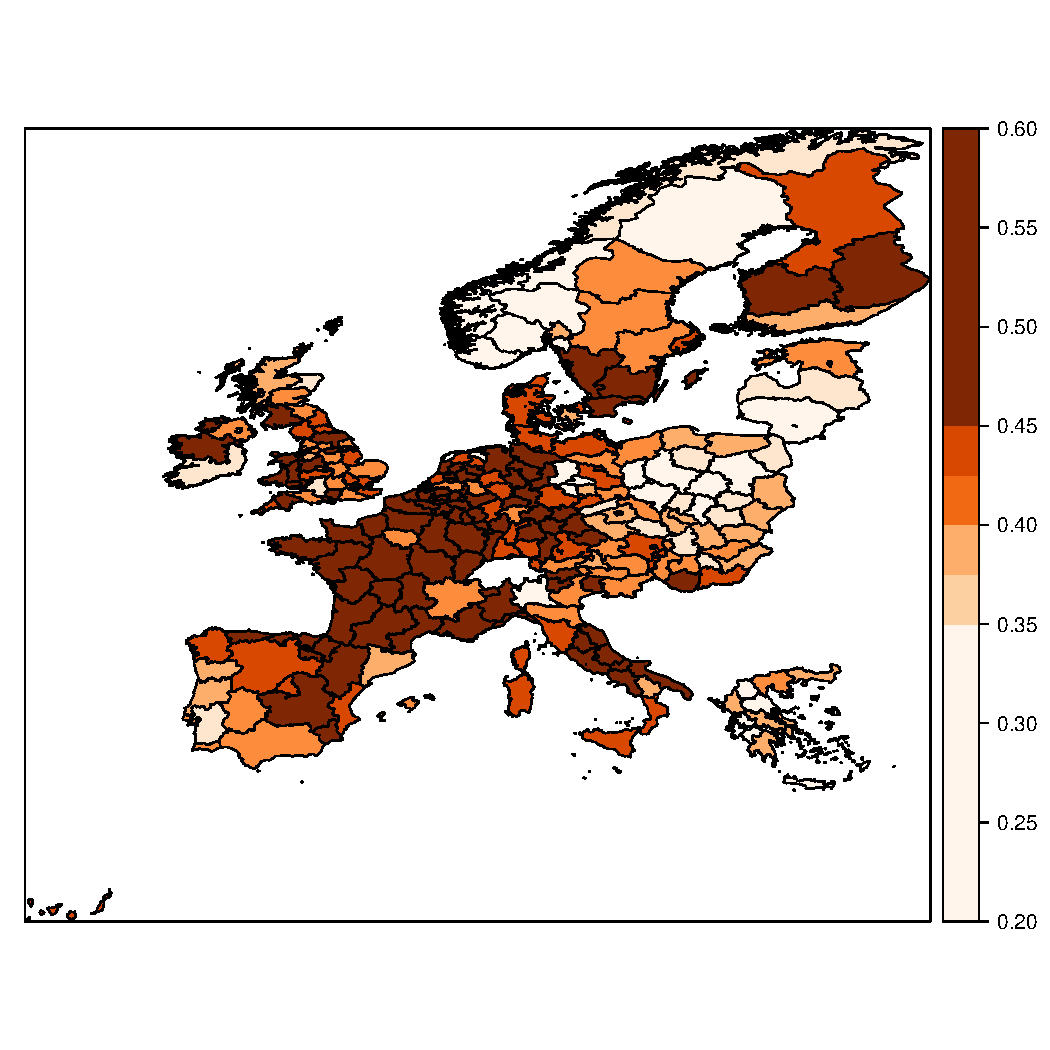
\includegraphics[width=0.75\textwidth]{TEfrontier}
\end{frame}

\begin{frame}{Regional efficiency manufacturing controlling for distance}
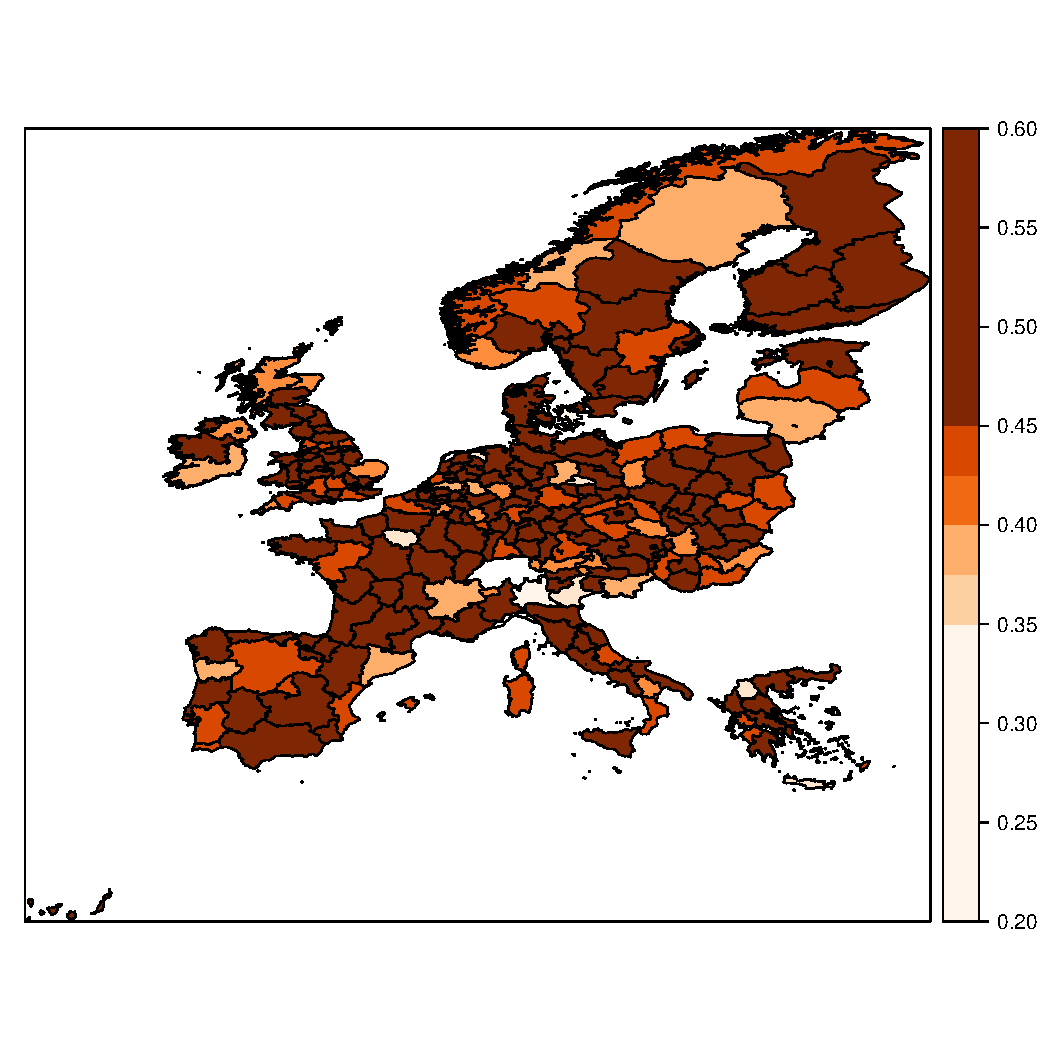
\includegraphics[width=0.75\textwidth]{TEfrontierError}
\end{frame}

\begin{frame}{Difference frontier vs. spatial error frontier for E \& M}
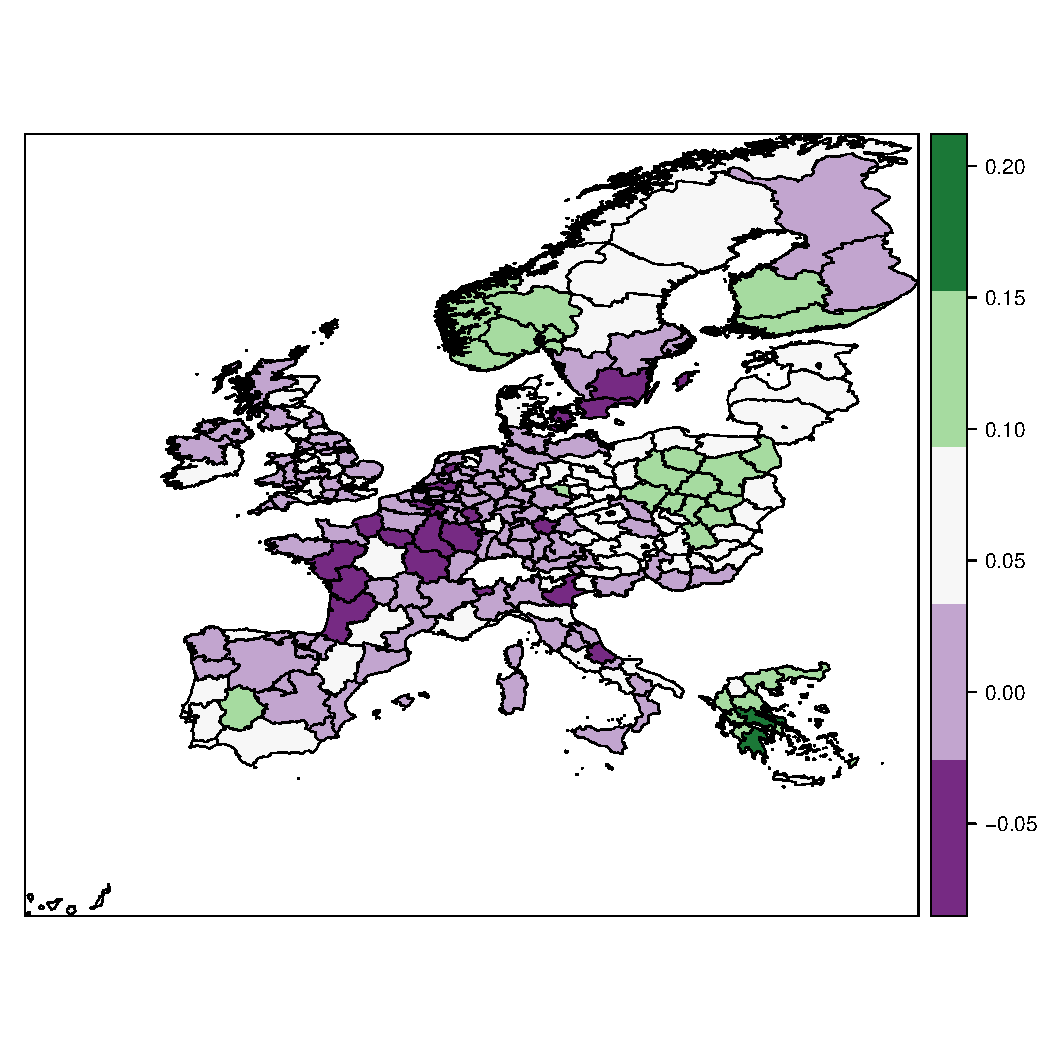
\includegraphics[width=0.75\textwidth]{TEfrontierdiff}
\end{frame}

\section{Conclusion}

\subsection{Conclusion \& further research}

\begin{frame}{In conclusion \& further research}

\end{frame}

\end{document}